\section{Annotation des sections et entités judiciaires}

\subsection{Objectif de la tâche}
\begin{frame}[t]{\mysubsectiontitle}
	Détecter les méta-données de référence et les normes

\begin{center}
	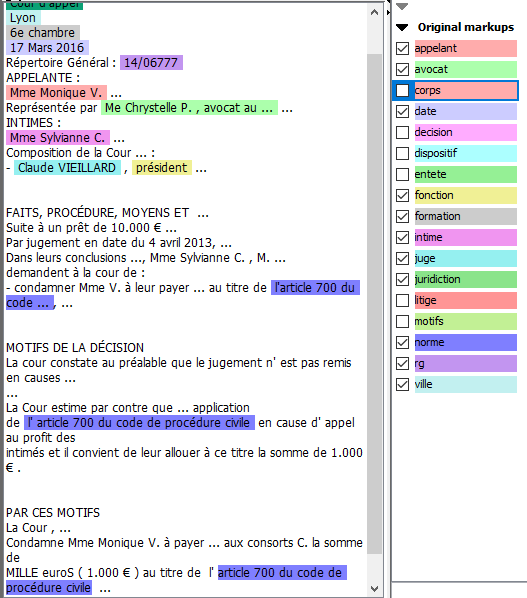
\includegraphics[height=0.8\textheight]{decision-marquee.png}
\end{center}

\end{frame}

\begin{frame}[t]{\mysubsectiontitle}
Sectionner pour organiser l'extraction des connaissances
\tiny
\begin{columns}\tiny
	\begin{column}{.45\linewidth}
		\fbox{\begin{minipage}{\textwidth}\textcolor{red}{Cour d'appel}
				 
				\textcolor{red}{Lyon}
				
				\textcolor{red}{6e chambre}
				
				\textcolor{red}{17 Mars 2016}
				
				Répertoire Général :  \textcolor{red}{14/06777}
				
				APPELANTE : 
				
				\textcolor{red}{Mme Monique V.}  ...
				
				Représentée par  \textcolor{red}{Me Chrystelle P. , 		
				avocat au ...}  ...
				
				INTIMES : 
				
				\textcolor{red}{Mme Sylvianne C.}  ...
				
				Composition de la Cour ... : 
				
				-  \textcolor{red}{Claude VIEILLARD}  ,  \textcolor{red}{président}  ...
		\end{minipage}}
		\vspace{0.1cm}
		
		{\textbf{Entête}: méta-données de référence de l'affaire}
		
		\vspace{0.4cm}
		
		\fbox{\begin{minipage}{\textwidth}PAR CES MOTIFS 
				
				La Cour , ...
				
				Confirme le jugement entrepris en toutes ses dispositions sauf en ce qu' il a ...
				
				Statuant à nouveau de ce chef , 
				
				Condamne Mme Monique V. à payer ... aux consorts C. la somme de 
				
				MILLE euroS ( \textcolor{red}{1.000 €} ) au titre de  l' \textcolor{red}{article 700 du code de procédure civile}  ...
		\end{minipage}}
		\vspace{0.1cm}
		
		{\textbf{Dispositif}: résultats et normes}
	\end{column}
	\begin{column}{.55\linewidth}
		\fbox{\begin{minipage}{\textwidth}
				\fbox{\begin{minipage}{0.95\textwidth}FAITS, PROCÉDURE, MOYENS ET  ...
						
						Suite à un prêt de 10.000 € ...
						
						Par jugement en date du 4 avril 2013, ...
						
						Dans leurs conclusions ..., Mme Sylvianne C. , M. ... 
						demandent à la cour de :
						
						- condamner Mme V. à leur payer ... au titre de  l'\textcolor{red}{article 700 du code ...} , ...
			\end{minipage}}		
			\vspace{0.1cm}
			
			{\textbf{Litige}: normes, faits, jugements antérieurs, prétentions et arguments des parties}
			
			\vspace{0.4cm}
			
			\fbox{\begin{minipage}{0.95\textwidth}MOTIFS DE LA DÉCISION 
					
					La cour constate au préalable que le jugement n' est pas remis en causes ...
					
					...
					
					La Cour estime par contre que ... application 
					de  l' \textcolor{red}{article 700 du code de procédure civile}  en cause d' appel au profit des 
					
					intimés et il convient de leur allouer à ce titre la somme de \textcolor{red}{1.000 €} . 
			\end{minipage}}		
			\vspace{0.1cm}
			
			{\textbf{Motifs}: normes, raisonnement des juges, réponses des juges}		 
		\end{minipage}}
		\vspace{0.1cm}
		
		{\textbf{Corps}}
						
	\end{column}
\end{columns}
\end{frame}

\subsection{Approches probabilistes de détection d'entités}
\begin{frame}[t]{\mysubsectiontitle}
Modèles probabilistes d'étiquetage de séquences

\scriptsize
\begin{table}[]
\begin{tabular}[]{c|c}
\toprule
{\textbf{HMM}} & {\textbf{CRF}} \\ \midrule
modèle génératif 	& modèle discriminant  \\
%\midrule		
%"\textbf{generate}" input	& {"\textbf{condition}" on input }\\%[0.25em]
\midrule
{un seul descripteur  par observation}	& {plusieurs descripteurs complexes par observation}\\%[0.25em]
\midrule	
\begin{tikzpicture}[->,>=stealth',shorten >=1pt,auto,node distance=1.3cm,
semithick]
\node[state] (S1)                    {$s_{t-1}$};
\node[state]         (S2) [right of=S1] 	  {$s_{t}$};
\node[state]         (O) [below of=S2] {$o_{t}$};
\path (S1) edge              node {} (S2)
(S2) edge              node {} (O);
\end{tikzpicture}
& 

\begin{tikzpicture}[auto,>=stealth',shorten >=1pt,auto,node distance=1.3cm,
semithick]
\node[state] (S1)                    {$s_{t-1}$};
\node[state]         (S2) [right of=S1] 	  {$s_{t}$};
\node[state]         (O) [below of=S2] {$o_{t}$};
\path (S1) edge              node {} (S2)
(S2) edge              node {} (O);
\end{tikzpicture}					
\\%[0.25em]
\midrule
$P(S,O) = \prod\limits_{t=1}^{T} P(s_t \vert s_{t-1}) P(o_t \vert s_{t})$  & $P_\lambda(S|O) = \frac{1}{Z(O)}exp\left( \sum\limits_{t=1}^{T}\sum\limits_{k} \lambda_k f_k(s_{t-1},s_t, o_t) \right) $ \\
% & & & \\
\tiny \cite{Seymore1999hmm} & \tiny \cite{peng2006crf} \\ 
\bottomrule
\end{tabular}
\end{table}

\normalsize
\end{frame}

\subsection{Sélection de modèles}
\begin{frame}[t]{\mysubsectiontitle}		
	Méthodes explorées
	
	\begin{itemize} \small
		\item Descripteurs de lignes pour les sections : 
		 \begin{itemize}
			\item forme : mots, longueur, etc. 
			\item contexte : position, lignes voisines, etc.
		 \end{itemize}
		\item Descripteurs de mots pour les entités : 
		\begin{itemize}
			\item forme : est-ce une initiale ("B.") ?,  un mot clé de norme ?, etc.
			\item contexte : mots voisins, position, etc.
			\item syntaxe : rôle grammaticale
		\end{itemize}
		\item Schéma d'étiquetage : distinction des parties d'une entité {\tiny
		\begin{tabular}{l|ccccccccc}
			& \textit{composée} & \textit{de} & \textit{Madame} & \textit{Martine} & \textit{JEAN} & , & \textit{Président} & \textit{de} & ... \\ 
			IO & O & O & I-JUGE & I-JUGE & I-JUGE & O & I-FONCTION & I-FONCTION & ... \\
			BIO & O & O & B-JUGE & I-JUGE & I-JUGE & O & B-FONCTION & I-FONCTION & ... \\
			IEO & O & O & I-JUGE & I-JUGE & E-JUGE & O & I-FONCTION & I-FONCTION & ...\\
			BIEO & O & O & B-JUGE & I-JUGE & E-JUGE & O & B-FONCTION & I-FONCTION & ... \\
		\end{tabular}}
		\item Approches de réduction du nombre de descripteurs
		\begin{itemize}
			\item recherche bidirectionnelle (BDS) \cite{liu2012featureSelection}
			\item sélection séquentielle avant à flottement (SFFS) \cite{pudil1994floatingFeatSelection}
		\end{itemize}
	\end{itemize}	
\end{frame}

\begin{frame}[t]{\mysubsectiontitle}
	Résultats (CRF)
	
	\begin{itemize}
		\item sélection du schéma d'étiquetage
		\begin{itemize}
			\item Les schémas plus complexes que IO rendent l'entraînement plus long
			\item Les schémas complexes ne semblent pas améliorer la détection des sections (baisse de $F_1$ de près de $20\%$)
			\item Les schémas complexes améliorent légèrement la détection d'entités de moins de $3\%$
		\end{itemize}
		\item sélection des descripteurs
		\begin{itemize}
			\item Lenteur des algorithmes BDS et SFFS (plus de 15h)
			\item BDS réduit de moitié
			\item SFFS réduit beaucoup plus
			\item Pas d'amélioration ou détérioration considérable de la détection
		\end{itemize}
	\end{itemize}
\end{frame}

\subsection{Discussions des résultats}
\begin{frame}[t]{\mysubsectiontitle}
	Confusions de labels (CRF)
	
	{}
\begin{columns}\tiny
	\begin{column}{.68\linewidth}
		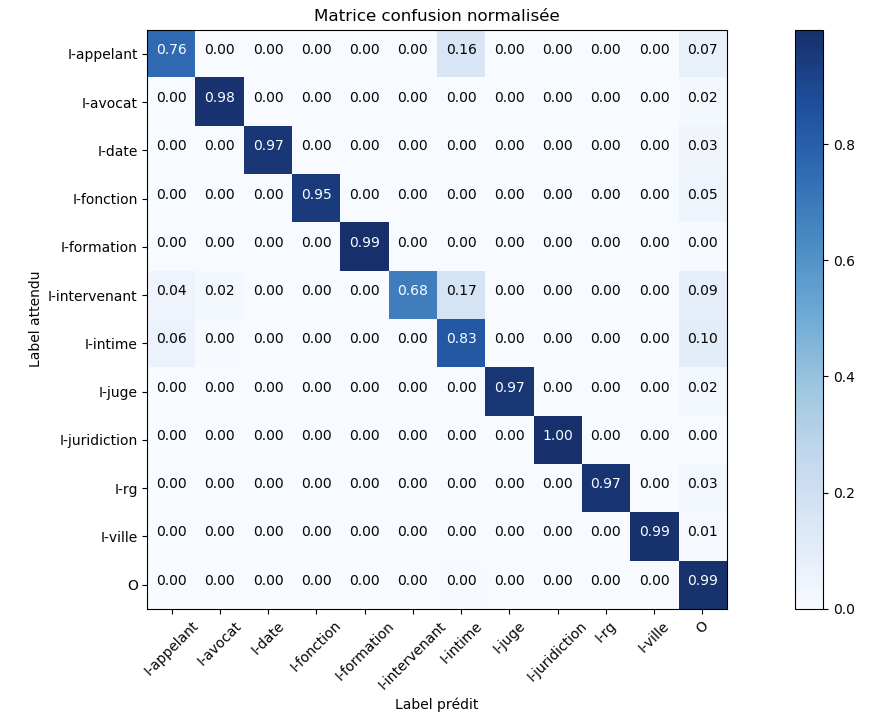
\includegraphics[width=\textwidth]{confusion_matrix_entete.png} 
	\end{column}
	\begin{column}{.3\linewidth}
		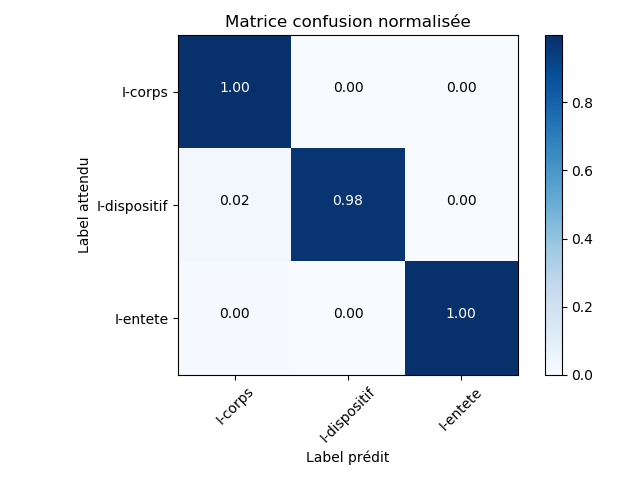
\includegraphics[width=\textwidth]{confusion_matrix_section.png}
	\end{column}
\end{columns}
\end{frame}

\begin{frame}[t]{\mysubsectiontitle}
	Impact de la quantité de décisions d'entraînement
	
\begin{figure}[!h]
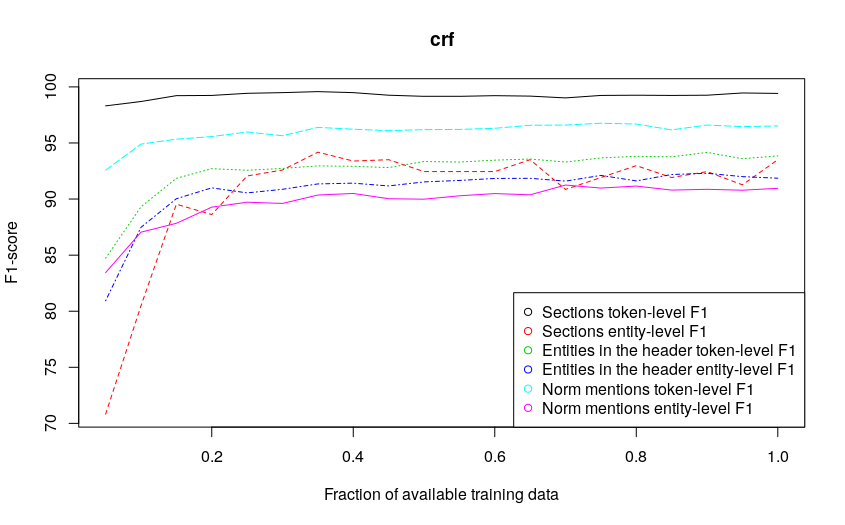
\includegraphics[width=0.9\textwidth]{lc-crf.png}
%\caption{Evolution de la F1-mesure en fonction de la fraction utilisée}\label{p4_crf-learning-curves}
\end{figure}
\end{frame}

\begin{frame}[t]{\mysubsectiontitle}
	Description manuelle vs. représentation apprise
	
\scriptsize
\begin{tabular}{|l|l|l|l|l|l|l|}
	\hline
	& \multicolumn{3}{c}{\textbf{CRF + descripteurs manuels}} & \multicolumn{3}{|c|}{\textbf{BiLSTM-CRF}} \\ \cline{2-7}
	& \textit{Precision} & \textit{Rappel}                     & $F_1$ & \textit{Precision} & \textit{Rappel} & $F_1$ \\ \hline
	\textbf{appelant}      & 82.49              & 69.42                               & 74.72       & 80.26              & 71.53                & 75.04       \\ 
	\textbf{avocat}        & 90.15              & 89.02                               & 89.56       & 84.93              & 87.88                & 86.36       \\ 
	\textbf{date}          & 95.34              & 91.46                               & 93.12       & 95.04              & 90.79                & 92.63       \\ 
	\textbf{fonction}      & 95.87              & 95.08                               & 95.44       & 92.69              & 93.48                & 93.03       \\ 
	\textbf{formation}     & 96.91              & 91.31                               & 93.7        & 91.05              & 89.47                & 89.84       \\ 
	\textbf{intervenant}   & 51.42              & 32.71                               & 36.8        & 31.48              & 20                   & 23.11       \\ 
	\textbf{intime}        & 76.01              & 79.15                               & 77.22       & 67.7               & 75.43                & 70.83       \\ 
	\textbf{juge}          & 95.67              & 94.07                               & 94.84       & 95.44              & 95.56                & 95.46       \\ 
	\textbf{juridiction}   & 98.55              & 98.25                               & 98.33       & 97.95              & 99.22                & 98.57       \\ 
	\textbf{rg}            & 95.46              & 95.29                               & 95.27       & 91.13              & 97.26                & 93.92       \\ 
	\textbf{ville}         & 98.33  & 93.01  & 94.71       & 91.43              & 95.34                & 93.3        \\ 
	\textbf{norme} & 91.08 & 90.27  & 90.67 & 91.43  & 92.65  & 92.03       \\ \hline
	\noalign{\smallskip}\hline\noalign{\smallskip}
	\textbf{Evaluation globale} & 92.2 & 90.09 & 91.12  & 89.21 & 90.43 & 89.81       \\ \hline
\end{tabular}
\end{frame}

\begin{frame}[t]{\mysubsectiontitle}
Sectionnement en 4 sections pour l'extraction des demandes

\centering
\begin{tabular}{|l|c|c|c|}
	\hline
	\multirow{2}{*}{}	&      \multicolumn{3}{|c|}{\textbf{CRF (\%)}}          \\ \cline{2-4} & \textit{Precision} & \textit{Rappel} & $F_1$ \\ \hline
	\textbf{entete} &   99.80 &	99.54 &	99.67      \\ 
	\textbf{litige}      &  96.10 &	97.66	& 96.87       \\ 
	\textbf{motifs}      &   97.31	&95.96	&96.62 \\
	\textbf{dispositif}    &   99.00&	98.49&	98.72  \\ \hline
	\textbf{Evaluation globale} &97.55	&97.55	&97.55       \\ \hline
\end{tabular}
\end{frame}
